\ifdefined\ishandout
\documentclass[handout]{beamer}
\else
\documentclass{beamer}
\fi

%\usepackage[frenchb]{babel}
\usepackage[T1]{fontenc}
%\usepackage[utf8]{inputenc}
\usepackage{hyperref}
\usepackage{multirow}
\usepackage{listings}
\usepackage{fancyvrb}
\usepackage{tikz}
\usepackage{framed}
\usepackage{xmpmulti}

\usepackage{algorithm}
\usepackage{algorithmicx}
\usepackage{algpseudocode}
\usepackage{xcolor}
\usepackage{booktabs}
\usepackage{color, colortbl}
\ifdefined\ishandout
\usepackage{handoutWithNotes}
\fi
\usepackage{slashbox}
\usepackage{amsmath}
\usepackage{bm}
\usepackage{hhline}
\usepackage{pgfplots}
\usepackage{caption}

\def\UrlBreaks{\do\/\do-}

\usetikzlibrary{shapes.geometric}
\usetikzlibrary{positioning}
\usetikzlibrary{shapes.arrows, chains}
\usetikzlibrary{arrows,calc}
\usetikzlibrary{shapes.multipart}
\usetikzlibrary{matrix}

\usepackage{array}
%\usetheme{Boadilla}
\usetheme[progressbar=frametitle]{metropolis}

\usefonttheme[onlymath]{serif}

\newcommand{\R}{\mathbb{R}}
%\newcommand{\C}{\mathbb{C}}
\newcommand{\N}{\mathbb{N}}
\newcommand{\Z}{\mathbb{Z}}
\newcommand{\E}{\mathbb{E}}
\newcommand{\Var}{\text{Var}}
\newcommand{\Cov}{\text{Cov}}
\ifdefined\ishandout
\pgfpagesuselayout{3 on 1 with notes}[a4paper,border shrink=5mm]
\usecolortheme{dove}
\else
%\usecolortheme{dolphin}
%\usecolortheme{crane}
\fi

\metroset{block=fill}

\lstnewenvironment{codeC}
{ \lstset{language=C,
    otherkeywords={printf,scanf}}
}
{}

\ifdefined\ishandout
\definecolor{mygreen}{rgb}{0,0,0}
\definecolor{mymauve}{rgb}{0,0,0}
\definecolor{myblue}{rgb}{0,0,0}
\else
\definecolor{mygreen}{rgb}{0,0.6,0}
\definecolor{mymauve}{rgb}{0.58,0,0.82}
\definecolor{myblue}{rgb}{0,0,1}

\fi

%% Notes
%\setbeameroption{show only notes}


\definecolor{mygray}{rgb}{0.5,0.5,0.5}

\lstset{ language=Python,%
  backgroundcolor=\color{white},   % choose the background color; you must add \usepackage{color} or \usepackage{xcolor}
  basicstyle=\footnotesize,        % the size of the fonts that are used for the code
  breakatwhitespace=false,         % sets if automatic breaks should only happen at whitespace
  breaklines=true,                 % sets automatic line breaking
  captionpos=b,                    % sets the caption-position to bottom
  commentstyle=\color{mygreen},    % comment style
  deletekeywords={...},            % if you want to delete keywords from the given language
  escapeinside={\%*}{*)},          % if you want to add LaTeX within your code
  extendedchars=true,              % lets you use non-ASCII characters; for 8-bits encodings only, does not work with UTF-8
  frame=tb,	                   % adds a frame around the code
  keepspaces=true,                 % keeps spaces in text, useful for keeping indentation of code (possibly needs columns=flexible)
  keywordstyle=\color{blue},       % keyword style
  otherkeywords={*,...},           % if you want to add more keywords to the set
  numbers=none,                    % where to put the line-numbers; possible values are (none, left, right)
  numbersep=5pt,                   % how far the line-numbers are from the code
  numberstyle=\tiny\color{mygray}, % the style that is used for the line-numbers
  rulecolor=\color{black},         % if not set, the frame-color may be changed on line-breaks within not-black text (e.g. comments (green here))
  showspaces=false,                % show spaces everywhere adding particular underscores; it overrides 'showstringspaces'
  showstringspaces=false,          % underline spaces within strings only
  showtabs=false,                  % show tabs within strings adding particular underscores
  stepnumber=2,                    % the step between two line-numbers. If it's 1, each line will be numbered
  stringstyle=\color{mymauve},     % string literal style
  tabsize=3,	                   % sets default tabsize to 2 spaces
  title=\lstname                   % show the filename of files included with \lstinputlisting; also try caption instead of title
}
%\lstset{language=Python,
% breakatwhitespace=false,         % sets if automatic breaks should only happen at whitespace
%  breaklines=true,                 % sets automatic line breaking
%  captionpos=b,                
%%commentstyle=\itshape\color{mymauve},
%%keywordstyle=\bfseries\color{myblue},
%numbers=left,                    % where to put the line-numbers; possible values are (none, left, right)
%  numbersep=8pt,                   % how far the line-numbers are from the code
%  numberstyle=\tiny\color{mygray}, % the style that is used for the line-numbers
%%  rulecolor=\color{black},         % if not set, the frame-color may be changed on line-breaks within not-black text (e.g. comments (green here))
%  showspaces=false,                % show spaces everywhere adding particular underscores; it overrides 'showstringspaces'
%%  showstringspaces=false,          % underline spaces within strings only
%  showtabs=false,                  % show tabs within strings adding particular underscores
%  stepnumber=2,                    % the step between two line-numbers. If it's 1, each line will be numbered
%%  stringstyle=\color{mygreen},     % string literal style
%  tabsize=2 
%}
\ifdefined\ishandout
\newcommand{\red}{\textbf}
\else
\newcommand{\red}{\textcolor{red}}
\fi
%\newcommand \emph
%Default size : 12.8 cm * 9.6 cm

\newcommand{\tmark}[1]{\tikz[remember picture, baseline=-.5ex]{\coordinate(#1);}}

\definecolor{bluegreen}{RGB}{0,149,182}


%\newcommand{\output}[1]{
\setbeamertemplate{navigation symbols}{}
\newcommand{\bvrb}{\Verb[commandchars=£µ§,formatcom=\color{bluegreen}]}
\newcommand{\footvrb}{\footnotesize\Verb}
\newcommand{\vrbalert}[2][]{\visible<#1>{#2}}
%%% Commande pour les listes/arbres
\newcommand{\mvide}{\nodepart{one} \nodepart{two}}
\newcommand{\tvide}{\nodepart{one} \nodepart{two} \nodepart{three}}
\newcommand{\rref}[1][]{\hfill{\scriptsize\textit{#1}}}

%%Fin des commandes pour les listes/arbres.



%%% Paramètres du cours (à régler)
%Numéro du cours
\newcommand{\nb}{1}

\title[Machine Learning]{Machine learning and physical modelling-2}
\author[J. Brajard]{julien.brajard@nersc.no}
\institute[NERSC]{NERSC\\
\url{https://github.com/brajard/MAT330}}
\date{October 2019}

\begin{document}
%%%%%%%%%%%%%%%%%%%%% SLIDES DE TITRE
\begin{frame}
\titlepage
%\centering{
%\url{http://australe.upmc.fr} (onglet EPU-C5-IGE Info Gen)}
\end{frame}

\begin{frame}{Table of contents}
  \setbeamertemplate{section in toc}[sections numbered]
  \tableofcontents[hideallsubsections]
\end{frame}

\section{Steps of a machine learning process}

\begin{frame}{Steps}
    \begin{figure}
        \centering
     \tikzstyle{block} = [rectangle, draw, fill=blue!20, text width=7em, text centered, rounded corners, minimum height=4em]
     \tikzstyle{line} = [draw, ->]
    \tikzstyle{back} = [draw, ->, very thick, red]
     
     \begin{tikzpicture}[auto, node distance=1cm and 2cm]
     \node[block] (collect) {Collect data} ;
     
     \pause
     \node [block, below= of collect] (feature) {Preprocess /clean data\\\footnotesize{\textit{feature extractions}}};
     \path [line] (collect)--(feature);

     \pause
     \node  [block, right= of collect] (tune) {Design model};
     
     \pause
     \node  [block, right= of feature] (train) {Train model};
     \path  [line] (feature)-- node[above]{train} (train);
     \path  [line] (tune)-- (train);
     
     \pause
     \node  [block, below= of train] (evaluate) {Evaluate model};
     \path  [line] (train)--(evaluate);
     \path  [line]  (feature) --  node[above,sloped]{(cross-)valid}(evaluate);

     \pause
     \path  [back]  (evaluate) edge[bend right=80] (tune);
     \path  [back]  (evaluate) edge[bend left] (feature);
     \path  [back]  (evaluate) edge[bend right] (collect);
     
     \pause
     \node  [block, fill=red!20, left=of evaluate]  (release) {Release model};
     \path  [line]  (evaluate)--(release);
     \path  [line]  (feature) -- node[above,sloped]{test} (release);

    

     \end{tikzpicture}
    \end{figure}
\end{frame}

%%%%%%%%%%%%%%%%%%%%%%%%%%%%%%%%%%%%%%%%%%
\begin{frame}{In summary}
    From one dataset, 3 sub-datasets have to be extracted:
    \begin{itemize}
        \item A training dataset
        \item A validation dataset
    \end{itemize}
    Can be done iteratively in a cross-validation procedure.\\
    \alert {Some parameters of the model (e.g. polynomial order in a polynomial regression) were determined from the validation dataset.}
    \begin{itemize}
        \item A test dataset (independent from the two other) to estimate the final performance of the model.
    \end{itemize}
\end{frame}

\section{A standard Machine learning model: Random Forests}

%%%%%%%%%%%%%%%%%%%%%%%%%%%%%%%%%%%%%%%%%%
\begin{frame}{A decision tree}
    Predict house price (in \$1000's) from 13 features:
    \begin{figure}
        \centering
        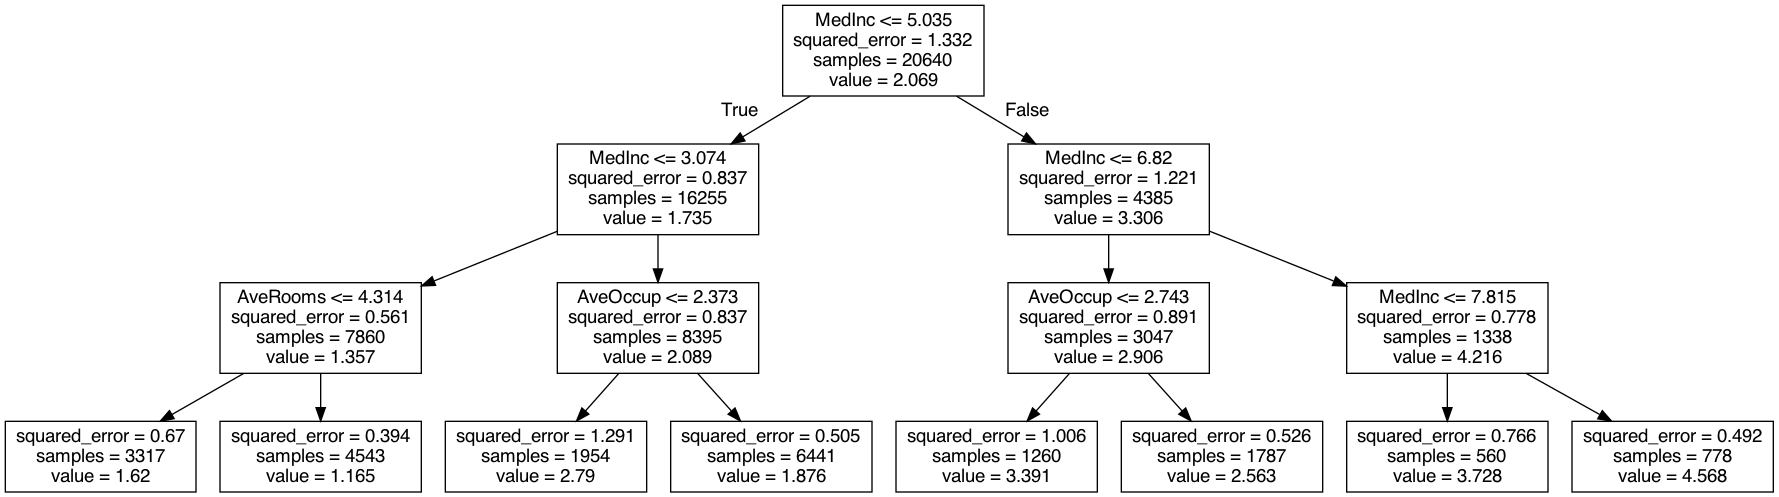
\includegraphics[width=.9\textwidth]{fig/L2/tree.png}
    \end{figure}
        
    \begin{table}
    \centering
    \begin{tabular}{c|l}
       CRIM   &  per capita crime rate by town \\   
       NOX    &  nitric oxides concentration  \\
       RM     &  average number of rooms per dwelling \\
       DIS    &  distance to employment centres \\
       LSTAT  &  lower status of the population \\
         
        \end{tabular}
        \end{table}

\end{frame}

%%%%%%%%%%%%%%%%%%%%%%%%%%%%%%%%%%%%%%%%%%
\begin{frame}{Uni-variate example}
\begin{columns}
\column{.5\textwidth}
\begin{figure}
    \centering
    \includegraphics<1>[width=\textwidth]{fig/L2/tree-data.png}
    \includegraphics<2>[width=\textwidth]{fig/L2/tree-2.png}
    \includegraphics<3>[width=\textwidth]{fig/L2/tree-5.png}
\end{figure}
    \column{.5\textwidth}
\begin{figure}
    \centering
    \includegraphics<2>[width=\textwidth]{fig/L2/tree_uni_2.png}
    \includegraphics<3>[width=\textwidth]{fig/L2/tree_uni_5.png}
\end{figure}
\end{columns}

\end{frame}

%%%%%%%%%%%%%%%%%%%%%%%%%%%%%%%%%%%%%%%%%%
\begin{frame}{From tree to forest}
Disadvantages of regression tree:
\begin{itemize}
    \item Can overfit the data
\end{itemize}
\visible<2->{
One extension of Regression Tree:
\alert{Random Forest}}
\begin{figure}
    \centering
    \includegraphics<1>[width=.7\textwidth]{fig/L2/tree.jpg}
    \includegraphics<2>[width=.7\textwidth]{fig/L2/forest.jpeg}
\end{figure}
\end{frame}

%%%%%%%%%%%%%%%%%%%%%%%%%%%%%%%%%%%%%%%%%%
\begin{frame}{The (over simplified) principle of Random Forest}
\begin{tikzpicture}[node distance = 0.5 cm]
\draw [very thick, fill=gray] (0,0) rectangle (3,6);
\node (data) at (1.5,6.2) {Data};
\pause
%TREE 1
\def\xx{4}
\def\yy{4.5}
\foreach \y in {0.5,2,3,3.5,4.5}
{
\draw[orange,fill=orange] (0,\y) rectangle +(3,.5);
}
\draw [very thick] (0,0) rectangle (3,6);

\draw [black,fill=orange] (\xx,\yy) rectangle +(1,1.5);
\path [->,draw] (3,3) -- (\xx,{\yy + 0.75});
\pause
\node [anchor=west] (t1) at ({\xx+2},{\yy + 0.75}) {Tree 1};
\path [->,draw] ({\xx+1},{\yy + 0.75}) -- node [above] {fit} ({\xx+2},{\yy + 0.75}) ;

\pause
%TREE 2
\def\xx{4}
\def\yy{2.5}

\draw [very thick, fill=gray] (0,0) rectangle (3,6);

\foreach \y in {0.,1,2,2.5,3.5,4.5}
{
\draw[blue,fill=blue] (0,\y) rectangle +(3,.5);
}
\draw [very thick] (0,0) rectangle (3,6);

\draw [black,fill=blue] (\xx,\yy) rectangle +(1,1.5);
\path [->,draw] (3,3) -- (\xx,{\yy + 0.75});
\node [anchor=west] (t2) at ({\xx+2},{\yy + 0.75}) {Tree 2};
\path [->,draw] ({\xx+1},{\yy + 0.75}) -- node [above] {fit} ({\xx+2},{\yy + 0.75}) ;

\pause
%TREE 3
\def\xx{4}
\def\yy{0.5}

\draw [very thick, fill=gray] (0,0) rectangle (3,6);

\foreach \y in {0.5,1.5,2,3.5,5.5}
{
\draw[red,fill=red] (0,\y) rectangle +(3,.5);
}
\draw [very thick] (0,0) rectangle (3,6);

\draw [black,fill=red] (\xx,\yy) rectangle +(1,1.5);
\path [->,draw] (3,3) -- (\xx,{\yy + 0.75});
\node [anchor=west] (t3)  at ({\xx+2},{\yy + 0.75}) {Tree 3};
\path [->,draw] ({\xx+1},{\yy + 0.75}) -- node [above] {fit} ({\xx+2},{\yy + 0.75}) ;

\pause
\node [right = of t2](average) {\textbf{Average}};
\node [right = of average] (out) {};
\path[->,draw] (t1) -- (average) ;
\path[->,draw] (t2) -- (average) ;
\path[->,draw] (t3) -- (average) ;
\path[->,draw] (average) -- (out) ;

\end{tikzpicture}
\end{frame}
%%%%%%%%%%%%%%%%%%%%%%%%%%%%%%%%%%%%%%%%%%
\begin{frame}{Results on the univariate experiment}

\begin{figure}
    \centering
\caption*{
\alt<1>{Prediction of Randoms trees}{Prediction of a Random Forest}}
    \includegraphics<1>[width=.9\textwidth]{fig/L2/tree-5.png}
    \includegraphics<2>[width=.9\textwidth]{fig/L2/RF.png}

\end{figure}


\end{frame}
%%%%%%%%%%%%%%%%%%%%%%%%%%%%%%%%%%%%%%%%%%
\begin{frame}[fragile]{Some key parameters}
\begin{lstlisting}[language=Python]
from sklearn.ensemble import RandomForestClassifier

rf = RandomForestRegressor(n_estimators=n, max_features=maxf, min_samples_split=min_split,...)
\end{lstlisting}
\vspace{-1.5em}
\begin{itemize}[<+->]
    \item \verb|n_estimators|: number of trees (generally the larger is the better)
    \item   \verb|max_features|: number of features to consider at each split. The default number is the total number of features. A larger value makes provides a smaller bias (accuracy) but a bigger variance (risk of overfitting)
      \item \verb|min_samples_fit|: number of features to consider at each split. The minimum value of 2 means that the tree is fully developed (small bias but great variance).
\end{itemize}

\end{frame}




%%%%%%%%%%%%%%%%%%%%%%%%%%%%%%%%%%%%%%%%%%
\begin{frame}{Determination of the hyperparameters}
    \begin{itemize}[<+->]
        \item Parameters that are not optimized during the training are called \alert{hyperparameters}.
        \item They can be determined using a score on the \alert{validation dataset} or using a \alert{cross-validation} procedure.
    \end{itemize}
    \pause
    \begin{columns}[b]
    \column{.42\textwidth}
      \begin{figure}
       \centering
       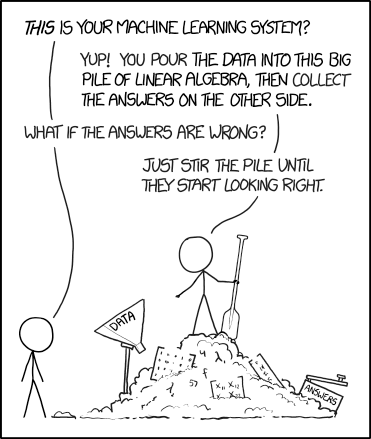
\includegraphics[width=\textwidth]{fig/L2/machine_learning.png}
   \end{figure}
   \column{.58\textwidth}
   \vfill
   {\footnotesize
   \url{https://xkcd.com/1838/}}
    \end{columns}

\end{frame}

%%%%%%%%%%%%%%%%%%%%%%%%%%%%%%%%%%%%%%%%%%
\begin{frame}{Stir the pile: The gridsearch}
\begin{enumerate}
    \item Specify a list of hyperparameters to be tested.
    \item For each of the parameters, specify a set of values to test
    \item Train a model for each of the possible combinations of hyperparameters
    \item Retain the best model (using, e.g., cross-validation)
\end{enumerate}

\begin{columns}[b]
\column{.5\textwidth}
\begin{figure}
    \centering
    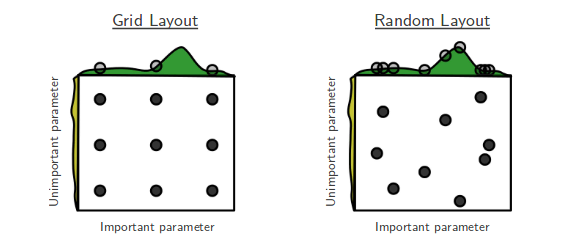
\includegraphics[trim={0 0 10cm 0},clip,width=\textwidth]{fig/L2/cIDuR.png}
\end{figure}
\column{.5\textwidth}

\vfill
{\footnotesize \url{https://medium.com/@senapati.dipak97/grid-search-vs-random-search-d34c92946318}
}
\end{columns}



\end{frame}

%%%%%%%%%%%%%%%%%%%%%%%%%%%%%%%%%%%%%%%%%%
\begin{frame}{Remarks on the gridsearch procedure}

\begin{itemize}[<+->]
    \item It make an \alert{exhaustive} search of the hyperparameters
    \item The procedure is easy to \alert{parallelized}.
    \item it is not naturally adapted for quantitative hyperparameters.
    \item it can become \alert{very costly}. (e.g. 8 hyperparameters with 8 values each to test = $8^8=16,777,216$ trainings.
\end{itemize}

\end{frame}


%%%%%%%%%%%%%%%%%%%%%%%%%%%%%%%%%%%%%%%%%%
\begin{frame}{Random search}
    \begin{enumerate}
    \item Specify a list of hyperparameters to be tested.
    \item For each of the parameters, specify a set of values to test or a law to draw a random value.
    \item Draw $n$ combinations of the hyperparameters.
    \item Train a model for each of the combinations.
    \item Retain the best model (using, e.g., cross-validation)
\end{enumerate}
\begin{figure}
    \centering
    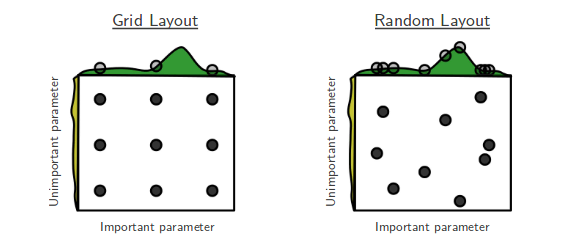
\includegraphics[width=.9\textwidth]{fig/L2/cIDuR.png}
\end{figure}
\end{frame}

%%%%%%%%%%%%%%%%%%%%%%%%%%%%%%%%%%%%%%%%%%
\begin{frame}{Remarks on the random search procedure}

\begin{itemize}
    \item It \alert{does not make} an \alert{exhaustive} search of the hyperparameters
    \item The procedure is easy to \alert{parallelized}.
    \item it is not adapted for quantitative hyperparameters.
    \item The cost is predictable (number of draw).
\end{itemize}
\pause
Both gridsearch and random search are implemented and easy to use in scikit-learn.
\end{frame}


\section{Feature processing}
%%%%%%%%%%%%%%%%%%%%%%%%%%%%%%%%%%%%%%%%%%
\begin{frame}[fragile]{Feature importance}
\begin{lstlisting}[language=Python]
rf = RandomForestRegressor(n_estimators=1000,max_features=10,random_state=10)
rf.fit(X,y)
importances = rf.feature_importances_
\end{lstlisting}
\vspace{-1.5em}
Indicates the impact of a feature in predicting the target.
\begin{columns}
\column{.5\textwidth}
    \begin{figure}
        \centering
        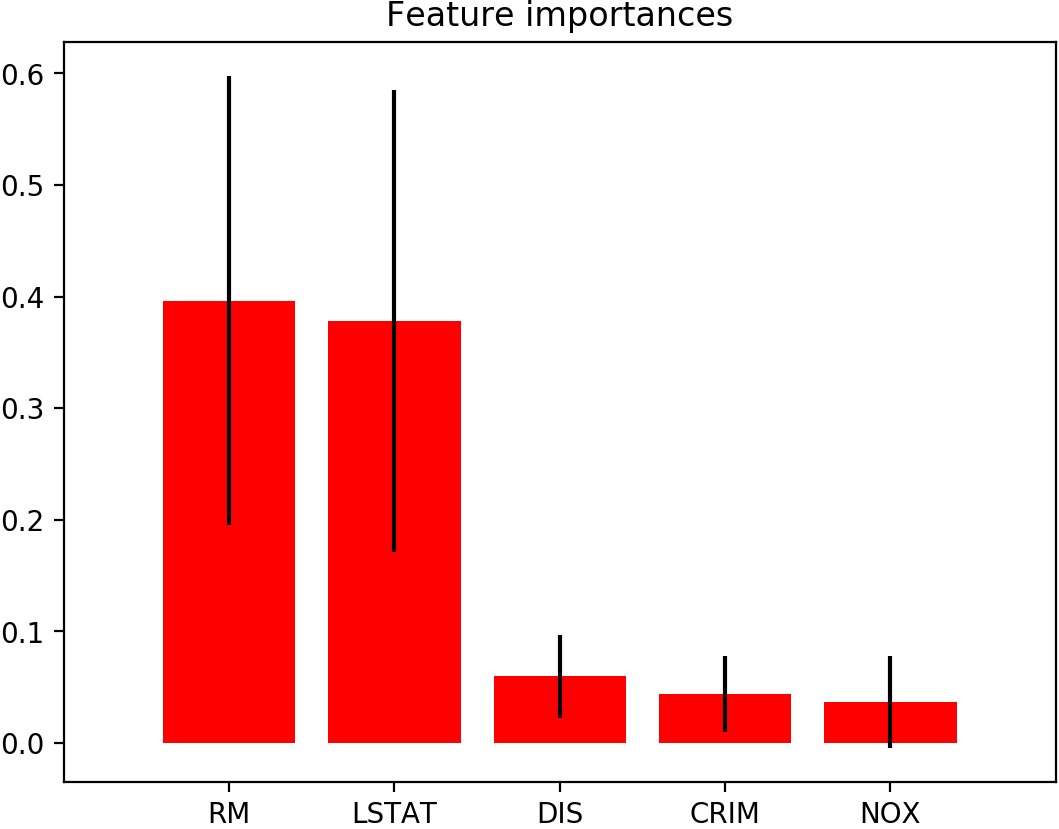
\includegraphics[width=.9\textwidth]{fig/L2/importance_RF.png}
    \end{figure}
\column{.5\textwidth}
    \begin{table}
    \centering
    \footnotesize
    \begin{tabular}{c|p{4.5cm}}
       CRIM   &  per capita crime rate by town \\   
       NOX    &  nitric oxides concentration  \\
       RM     &  average number of rooms per dwelling \\
       DIS    &  distance to employment centres \\
       LSTAT  &  lower status of the population \\
         
        \end{tabular}
        \end{table}

\end{columns}
\end{frame}

\begin{frame}{Type of features}
    \begin{itemize}[<+->]
        \item quantitative/continuous features (e.g. distance to employment centres, temperature)
        \item ordinal/discrete features (e.g. number of rooms, category of an hurricane)
        \item categorical features (e.g. name of the neighbourhood, name of the ocean)
    \end{itemize}
    \pause
    \begin{alertblock}{Encoding of the features?}
    
    \end{alertblock}
    
\end{frame}

\begin{frame}{Feature encoding}
\begin{table}[]
    \centering
    \footnotesize
    \begin{tabular}{|p{.15\textwidth}|p{.1\textwidth}|p{.33\textwidth}|p{.31\textwidth}|}
         Type  & \multicolumn{2}{c|}{Examples} & Encoding \\
         \hline
         Quantitative & distance & $\{1.2, 2.3, 0.1\}$ & $\{1.2, 2.3, 0.1\}$\\
                  \hline
         Ordinal & rooms & $\{2,3,4\}$ & $\{2,3,4\}$ \\
                  \hline
        Qualitative & Ocean & $\{{\rm Atlantic, Indian, Pacific}\}$ & $\{[1,0,0], [0,1,0], [0,0,1]\} $\\
        \hline
    \end{tabular}

\end{table}
\pause
Qualitative variable: one-hot encoding.
\begin{itemize}

    \item You must \alert{not} encode qualitative features with integer $1,2,3$, it would mean that Pacific > Indian > Atlantic.
    \item In {\rm sklearn} there is a function that makes the one-hot encoding: {\rm OneHotEncoder()}

    \item If the number of modalities (number of different features) is high, encoding qualitative feature produce a big-sized vector.
\end{itemize}
\end{frame}

\begin{frame}{Embedding}
    A common way to deal with features with a lot of modalities : \alert{Embedding}
    
    \begin{block}{Principle of embedding}
    Let's consider a qualitative variable with $n$ modalities, represented by the n-dimensional binary vector ${\bf x}$ 
    
    Embedding consists in representing this variable by a vector ${\bf v} \in \mathbb{R}^p, p << n$
    
    The embedding is represented by a matrix ${\bf M} \in \mathbb{R}^{n\times p}$ such as:
    $$
    {\bf v} = {\bf M}\cdot{\bf x}
    $$
    \end{block}
    Coefficients of ${\bf M}$ have to be optimized given an objective criteria (that depends on your problem)
    
\end{frame}

%%%%%%%%%%%%%%%%%%%%%%%%%%%%%%%%%%%%%%%%%%
\begin{frame}{one example: word cloud}
On the introduction of the \textit{Goodfellow et al.} book.\\
${\rm v}$ is 3-dimensional ($x$,$y$,size)
\begin{figure}
    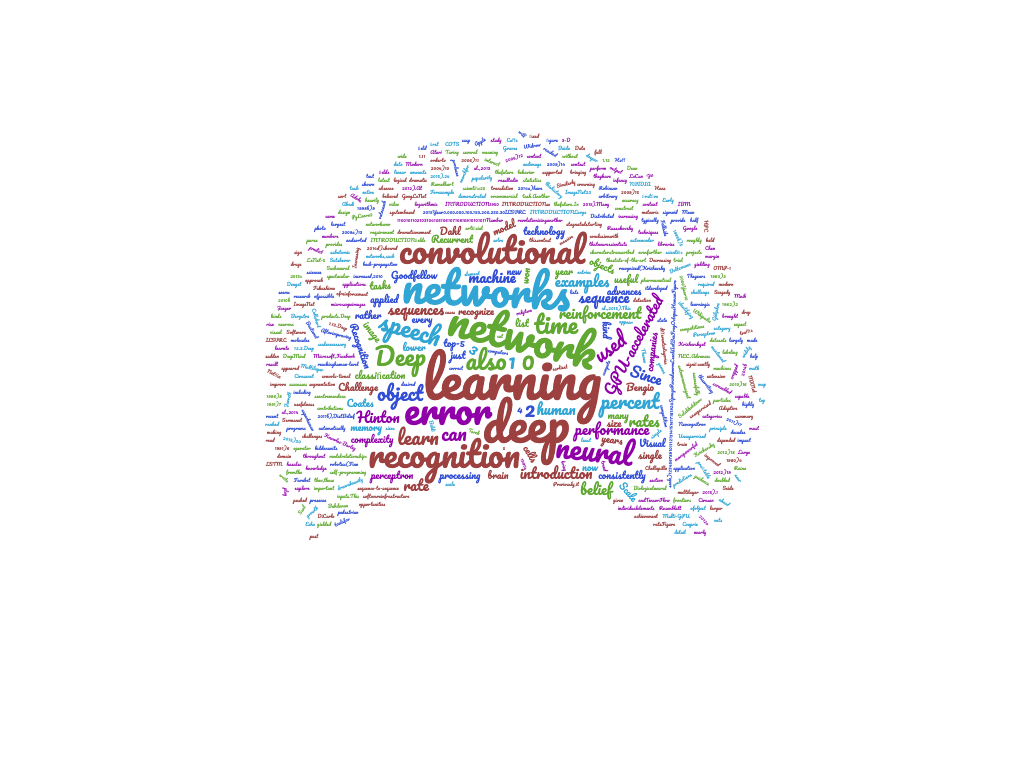
\includegraphics[trim={2cm 5cm 2cm 5cm},clip,width=\textwidth]{fig/L2/wordcloud.png}
\end{figure}
{\footnotesize
\href{https://www.wordclouds.com}{https://www.wordclouds.com}}
\end{frame}

%%%%%%%%%%%%%%%%%%%%%%%%%%%%%%%%%%%%%%%%%%
\section{Neural Networks}

\begin{frame}
  \frametitle{The perceptron : an artificial neuron}
  \begin{tikzpicture}[
    basic/.style={draw,fill=blue!20,text width=1em,text badly centered},
    input/.style={basic,circle},
    weights/.style={basic,rectangle},
functions/.style={basic,circle,fill=blue!10},
]
        \node[functions] (center) {};
        \node[below of=center,font=\scriptsize,text width=4em] {Activation function};
        \draw[thick] (0.5em,0.5em) -- (0,0.5em) -- (0,-0.5em) -- (-0.5em,-0.5em);
      %  \draw (0em,0.75em) -- (0em,-0.75em);
      %  \draw (0.75em,0em) -- (-0.75em,0em);
        \node[right of=center, anchor = west] (right) {$y=$ 0 ou 1};
            \path[draw,->] (center) -- (right);
        \node[functions,left=3em of center] (left) {$\sum$};
            \path[draw,->] (left) -- (center);
%        \node[weights,left=3em of left] (2) {$w_2$} -- (2) 
            \node[input,left= 4em of left] (l2) {$x_2$};
%            \path[draw,->] (l2) -- (2);
            \path[draw,->] (l2) -- node[above,midway]{$w_2$}(left);
        \node[below of=l2] (dots) {$\vdots$} ;
%(dots) node[left of=dots] (ldots) {$\vdots$};
%        \node[weights,below of=dots] (n) {$w_n$} -- (n) 
\node[input,below of=dots] (ln) {$x_n$};
%            \path[draw,->] (ln) -- (n);
            \path[draw,->] (ln) -- node[above,midway]{$w_n$}(left);
%        \node[weights,above of=2] (1) {$w_1$} -- (1) 
            \node[input,above of=l2] (l1) {$x_1$};
%            \path[draw,->] (l1) -- (1);
            \path[draw,->] (l1) -- node[above,midway]{$w_1$}(left);
%        \node[weights,above of=1] (0) {$w_0$} -- (0) 
\node[input,above of=l1] (l0) {$1$};
%            \path[draw,->] (l0) -- (0);
            \path[draw,->] (l0) -- node[above,midway]{$w_0$}(left);
        \node[below of=ln,font=\scriptsize](lin) {inputs};
        \node[right of=lin,xshift=+1em,font=\scriptsize] {weights};
    \end{tikzpicture}
\begin{block}{Computation}
$
y = f\left( w_0 + w_1. x_1 + w_2. x_2 +  \dots + w_n. x_n \right) = f\left( w_0 + \sum_{i=1}^n w_i.x_i\right)
$
\end{block}
\end{frame}

\begin{frame}{Some remarks}
\begin{itemize}[<+->]
    \item Inputs $x_i$ are the different features of the data
    \item Weight $w_i$ are the parameters of the model to optimize
    \item If the activation function is identity, it is equivalent to a linear regression
\end{itemize}
\visible<4->{
\begin{block}{}
More complexe models are build by combining several perceptrons
\end{block}
}

\end{frame}


\begin{frame}{Multi-layer perceptron (Densely connected layers)}
    \def\layersep{1.5cm}

\begin{tikzpicture}[
   shorten >=1pt,->,
   draw=black!50,
    node distance=\layersep,
    every pin edge/.style={<-,shorten <=1pt},
    neuron/.style={circle,fill=black!25,minimum size=17pt,inner sep=0pt},
    input neuron/.style={neuron, fill=green!50},
    output neuron/.style={neuron, fill=red!50},
    hidden neuron/.style={neuron, fill=blue!50},
    annot/.style={text width=4em, text centered}
]

    % Draw the input layer nodes
    \foreach \name / \y in {1,...,4}
    % This is the same as writing \foreach \name / \y in {1/1,2/2,3/3,4/4}
        \node[input neuron, pin=left:Feature \#\y] (I-\name) at (0,-\y) {};

    % set number of hidden layers
    \newcommand\Nhidden{3}

    % Draw the hidden layer nodes
    \foreach \N in {1,...,\Nhidden} {
       \foreach \y in {1,...,5} {
          \path[yshift=0.5cm]
              node[hidden neuron] (H\N-\y) at (\N*\layersep,-\y cm) {};
           }
    \node[annot,above of=H\N-1, node distance=1cm] (hl\N) {Hidden layer \N};
    }

    % Draw the output layer node
    \node[output neuron,pin={[pin edge={->}]right:Output}, right of=H\Nhidden-3] (O) {};

    % Connect every node in the input layer with every node in the
    % hidden layer.
    \foreach \source in {1,...,4}
        \foreach \dest in {1,...,5}
            \path (I-\source) edge (H1-\dest);

    % connect all hidden stuff
    \foreach [remember=\N as \lastN (initially 1)] \N in {2,...,\Nhidden}
       \foreach \source in {1,...,5}
           \foreach \dest in {1,...,5}
               \path (H\lastN-\source) edge (H\N-\dest);

    % Connect every node in the hidden layer with the output layer
    \foreach \source in {1,...,5}
        \path (H\Nhidden-\source) edge (O);

    % Annotate the layers

    \node[annot,left of=hl1] {Input layer};
    \node[annot,right of=hl\Nhidden] {Output layer};
\end{tikzpicture}
\end{frame}

\begin{frame}{Most usual activation functions}
\begin{columns}
\column{.5\textwidth}
    \begin{figure}
        \centering
        Linear\\
        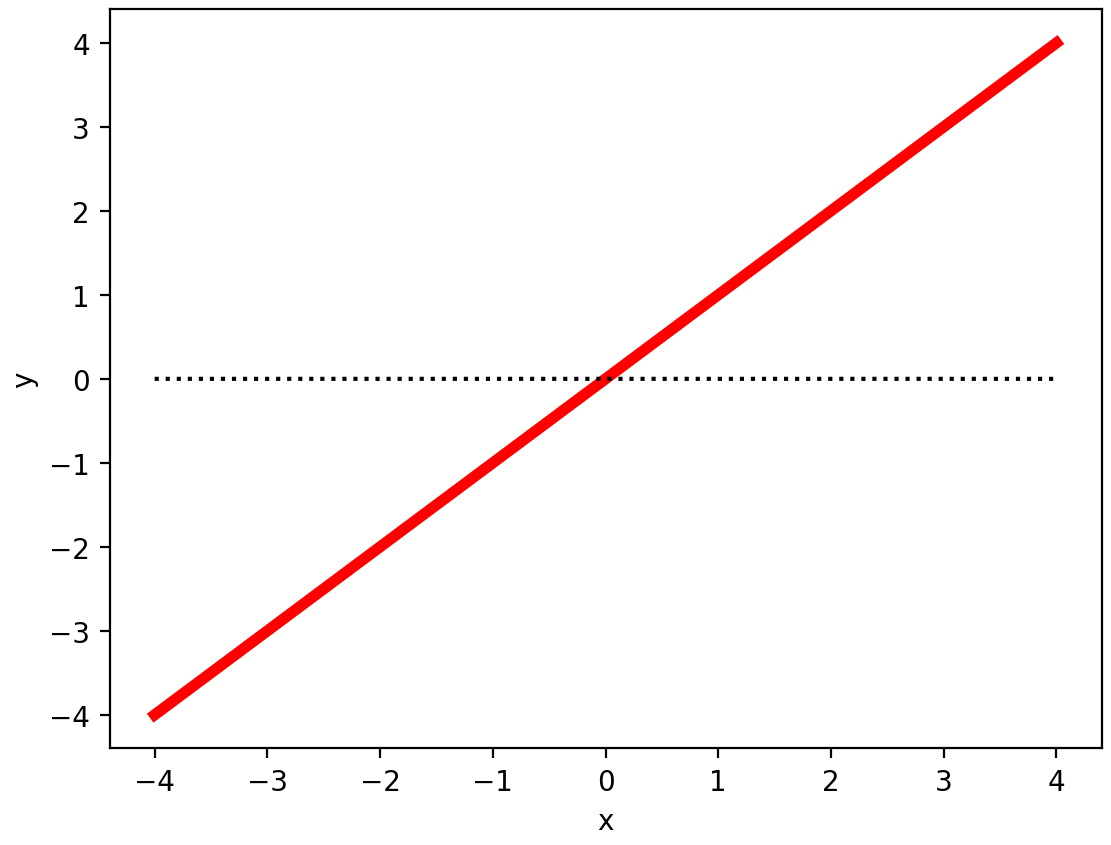
\includegraphics[width=.85\textwidth]{fig/L2/activ-linear.png}\\
        ReLU\\
        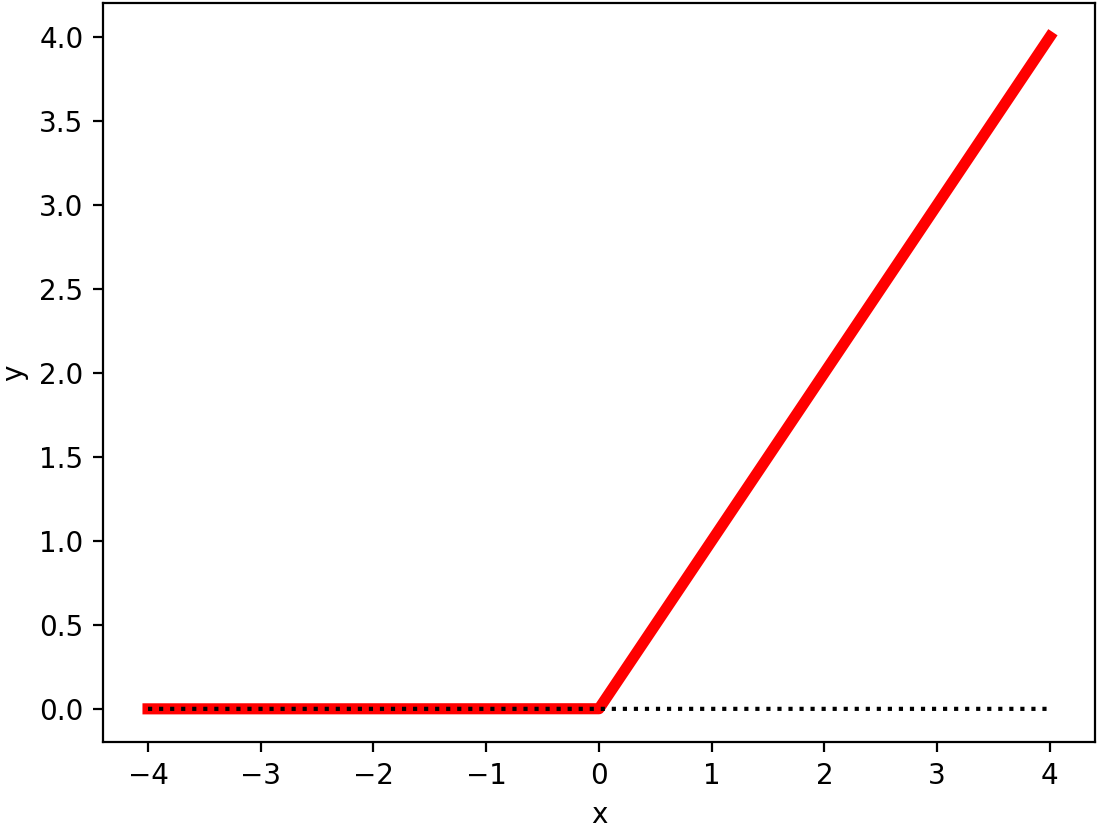
\includegraphics[width=.85\textwidth]{fig/L2/activ-relu.png}\\

    \end{figure}
\column{.5\textwidth}
    \begin{figure}
     \centering
        Hyperbolic tangent\\
        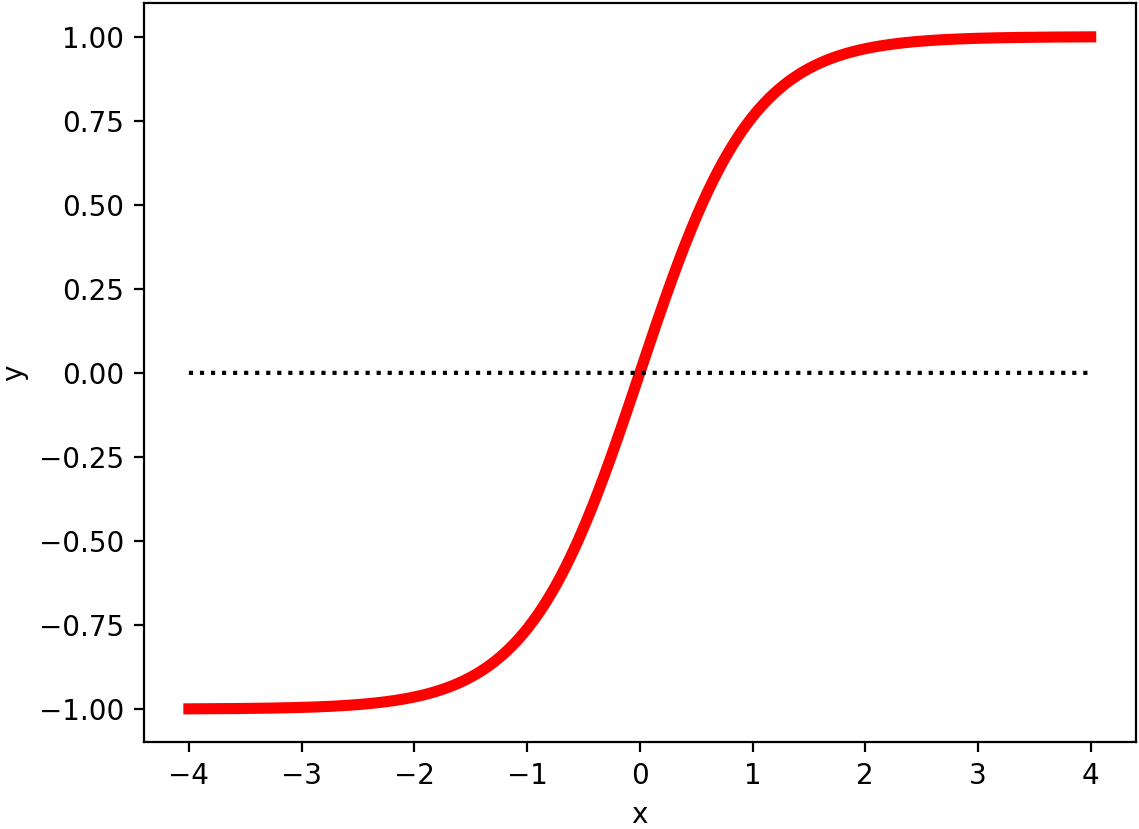
\includegraphics[width=.85\textwidth]{fig/L2/activ-tanh.png}\\
       Sigmoid\\
        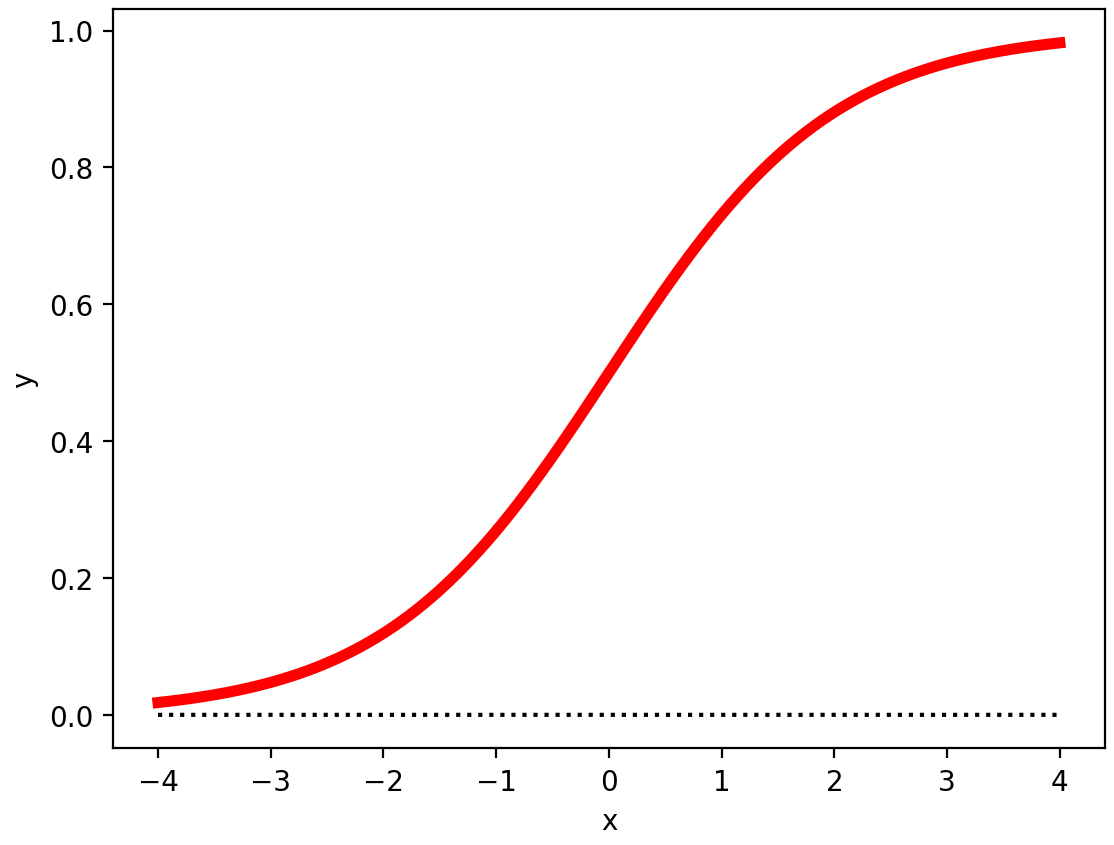
\includegraphics[width=.85\textwidth]{fig/L2/activ-sigmoid.png}\\

    \end{figure}
\end{columns}
\end{frame}


\begin{frame}{New fancy activation functions}
\begin{columns}
\column{.5\textwidth}
    \begin{figure}
        \centering
        Leaky-ReLU\\
        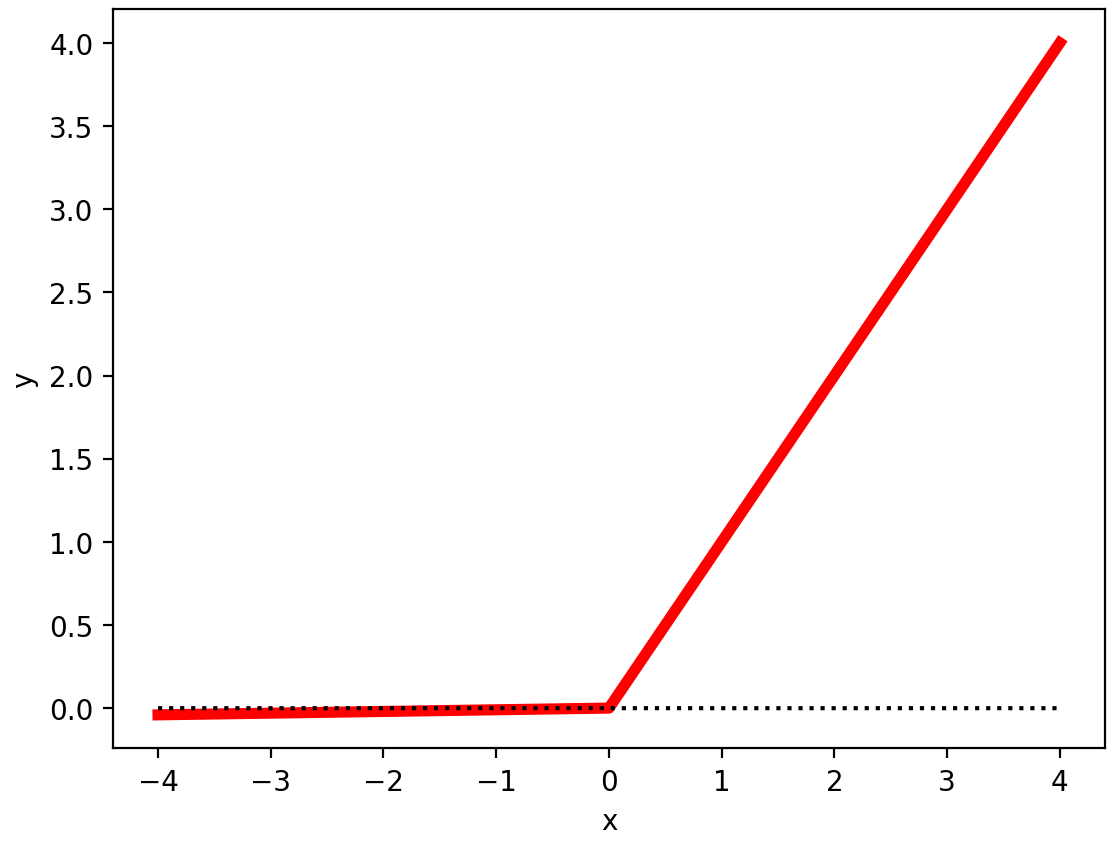
\includegraphics[width=.85\textwidth]{fig/L2/activ-l-relu.png}\\
      

    \end{figure}
\column{.5\textwidth}
    \begin{figure}
     \centering
        Swish\\
        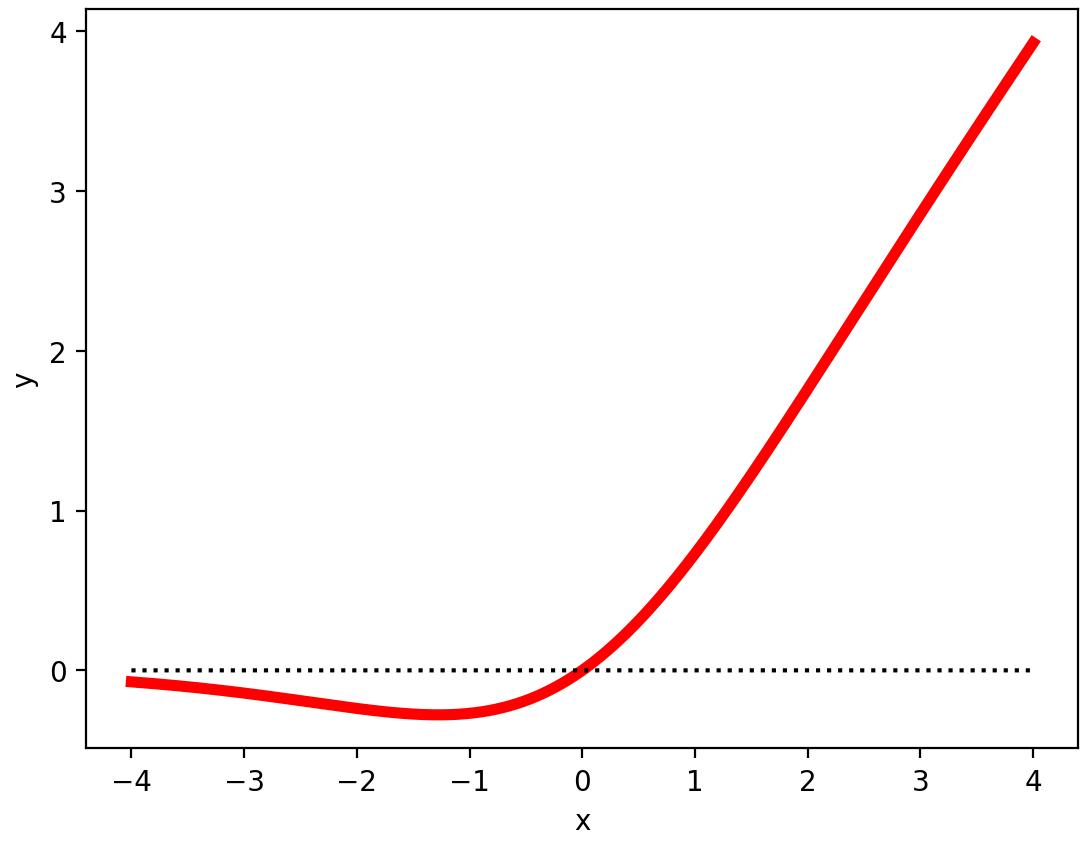
\includegraphics[width=.85\textwidth]{fig/L2/activ-swish.png}\\
     

    \end{figure}
\end{columns}
\end{frame}


\begin{frame}{Classification and regression loss}
  
   \begin{columns}
   \column{.5\textwidth}
   \alert{Regression}
   \begin{itemize}
       \item Last layer:\\
       linear or hyperbolic tangent
       \item Loss function:\\
       $$L(\hat{y},y) = \sum_i (\hat{y}_i-y_i)^2$$
   \end{itemize}
   \pause
\column{.5\textwidth}
       \alert{Classification}
   \begin{itemize}
       \item Last layer:\\
       Soft-max
       $$
       p_j=f_j(\mathbf{h}) = \frac{e^{h_j}}{\sum_k e^{h_k}}
       $$
       
       \item Loss function:\\
       Negative crossentropy
       $$L(p,y) = -\sum_i \sum_j y_{i,j}.\log{p_{i,j}}$$
   \end{itemize}
   \end{columns}
\end{frame}

\begin{frame}[fragile]{Convolutional neural net}
    \begin{tikzpicture}
    \draw[step=0.8,color=gray] (0,0) grid (4.8,4.8);
    \matrix[matrix of nodes,
    inner sep=0pt,
    anchor=south west,
    nodes={inner sep=0pt,text width=.8cm,align=center,minimum height=0.8cm}
    ]{
    $x_{11}$ & $x_{12}$ & $x_{13}$& $x_{14}$ & $x_{15}$  & $x_{16}$ \\
     $x_{21}$ & $x_{22}$ & $x_{23}$& $x_{24}$ & $x_{25}$ &  $x_{26}$ \\
    $x_{31}$ &$x_{32}$ & $x_{33}$& $x_{34}$ & $x_{35}$  & $x_{36}$ \\
    $x_{41}$ &$x_{42}$ & $x_{43}$& $x_{44}$ & $x_{45}$ & $x_{46}$  \\
     $x_{51}$ &$x_{52}$ & $x_{53}$& $x_{54}$ & $x_{55}$&  $x_{56}$  \\
     $x_{61}$ &$x_{62}$ & $x_{63}$& $x_{64}$ & $x_{65}$&  $x_{66}$  \\
    };
    \node (in) at (4.8,2.4) {} ;
    \node (out) at (8,2.4) {} ;
    \draw[step=0.8,color=gray] (8,0.8) grid (11.2,4);
    \matrix[matrix of nodes,
    xshift=8cm,
    yshift=0.8cm,
    inner sep=0pt,
    anchor=south west,
    nodes={inner sep=0pt,text width=.8cm,align=center,minimum height=0.8cm}
    ]{
    $h_{11}$ & $h_{12}$ & $h_{13}$& $h_{14}$ \\
     $h_{21}$ & $h_{22}$ & $h_{23}$& $h_{24}$ \\
    $h_{31}$ &$h_{32}$ & $h_{33}$& $h_{34}$   \\
    $h_{41}$ &$h_{42}$ & $h_{43}$& $h_{44}$  \\
    };
    
    \draw[step=0.5,color=gray] (5.999,3.499) grid (7.5,5);
    \matrix[matrix of nodes,
    xshift=5.999cm,
    yshift=3.499cm,
    inner sep=0pt,
    anchor=south west,
    nodes={inner sep=0pt,fill=orange!20,font=\footnotesize,text width=.5cm,align=center,minimum height=0.5cm}
    ]{
    $w_{11}$ & $w_{12}$ & $w_{13}$ \\
    $w_{21}$ & $w_{22}$ & $w_{23}$ \\
    $w_{31}$ & $w_{32}$ & $w_{33}$ \\
    };
    
    \path [draw, very thick, ->] (in) edge[bend left=40] 
    node [above,midway]{$\mathbf{w}$}(out);
    \node (xlabel) at (2.4,5) {$X$: an image};
    \node (hlabel) at (9.6,4.2) {$h$: first feature};
    \end{tikzpicture}
    \begin{block}{Perform a standard convolution}
    $$
    h_{i,j} = \sum_{k=1}^3\sum_{l=1}^3 x_{i+k-1,j+l-1}.w_{k,l}
    $$
    \end{block}
\end{frame}


\begin{frame}[t]{Main parameters of a convolutional layer}
\begin{itemize}
    \item <1-> \alert<1> {Size of the filter} $K$ 
    \item <2-> \alert<2> {Number of filters} $p$

\only<2>{
A convolutional layer is composed of $p$ convolutions (size of layer) extracting $p$ features from the data.
\begin{figure}
\centering
    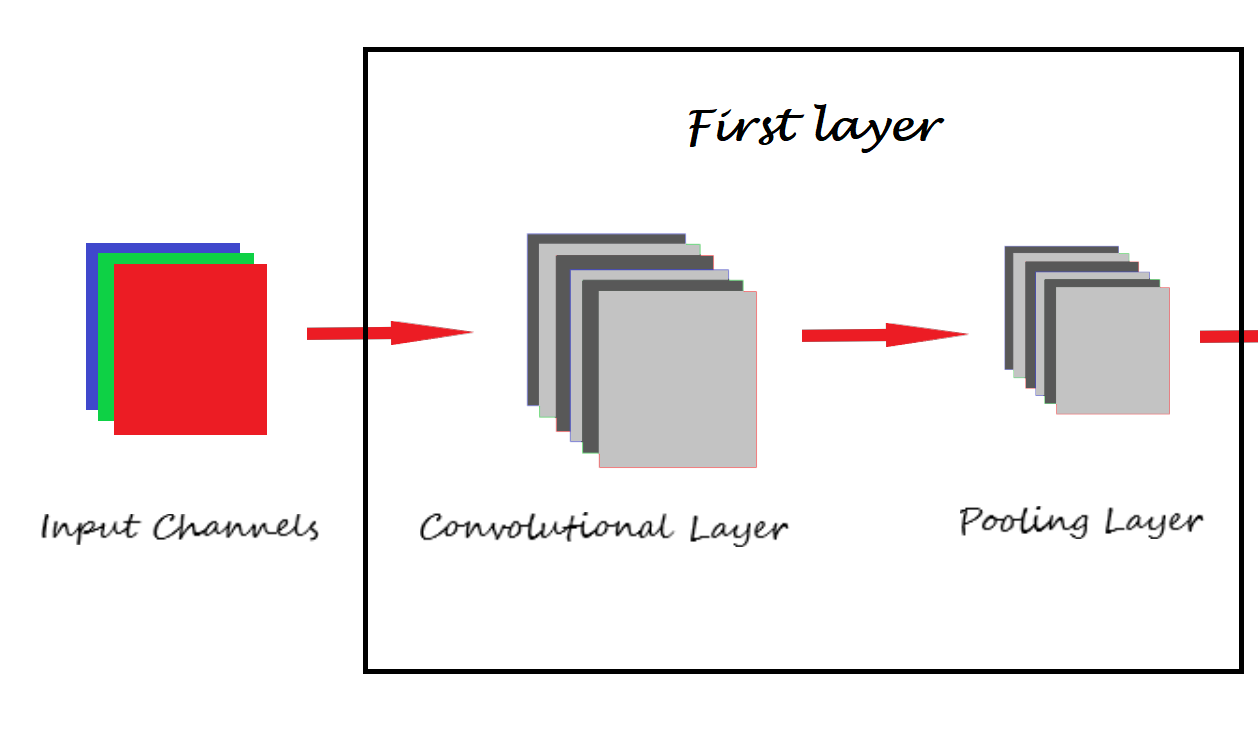
\includegraphics[width=.6\textwidth,trim={0 3.5cm 12.5cm 5cm},clip]{fig/L2/Cnn-layer.png}
\end{figure}
}

    \item <3-> \alert<3> {Strides} $S$
    
    \only<3> {
{\centering
\begin{tabular}{cc}
    $S=1$ & $S=2$ \\
    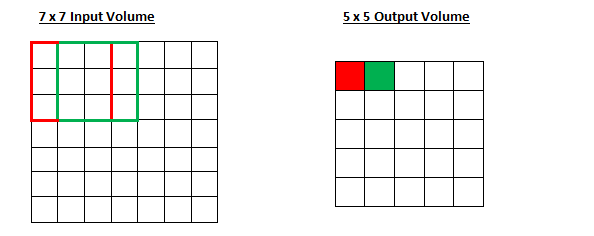
\includegraphics[trim={0.5cm 0 2.5cm 0}, clip, width=.5\textwidth]{fig/L2/Stride1.png}&
    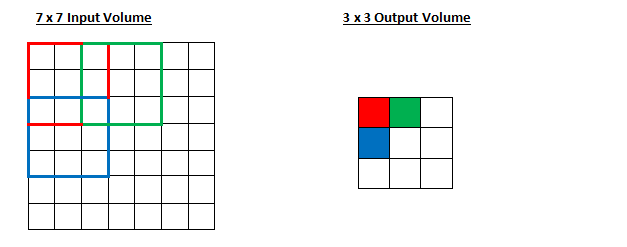
\includegraphics[trim={0 0 2.5cm 0}, clip, width=.5\textwidth]{fig/L2/Stride2.png}\\
    \end{tabular}
    }}
    
    \item <4-> \alert<4> {Padding} $P$
    
    {\only<4>
    {\centering
\begin{tabular}{cc}
    $P=1$ & $P=2$ \\
    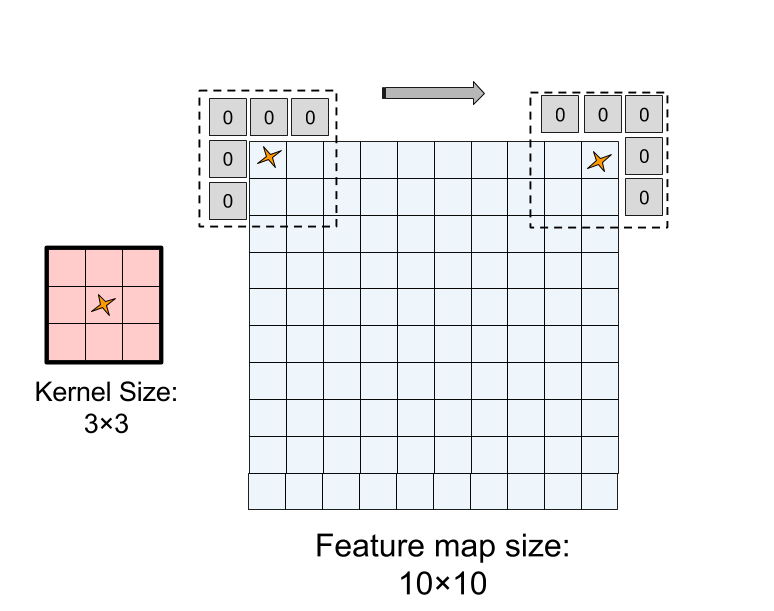
\includegraphics[trim={0 0 1.5cm 0}, clip, width=.45\textwidth]{fig/L2/pad3.png}&
    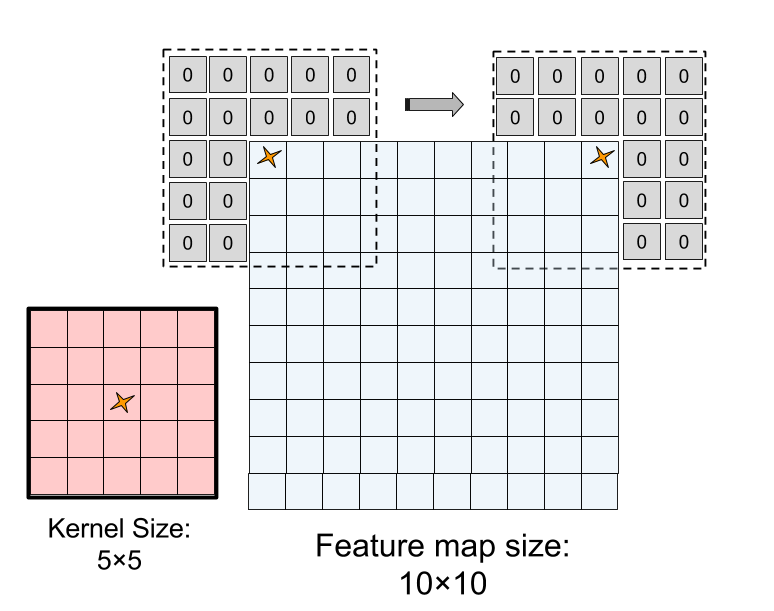
\includegraphics[trim={0 0 1.5cm 0}, clip, width=.45\textwidth]{fig/L2/pad5.png}\\
    \end{tabular}
    }

}
    
\end{itemize}
    \pause
    {\footnotesize
    $O = \frac{W - K +2P}{S} + 1$, where $O$ is the output size and $W$ the input size.
    }
\end{frame}


\begin{frame}{Summary of Convolutional layer steps}
    \begin{figure}
        \centering
        1. Convolution
\multiinclude[<+->][format=png,graphics={width=\textwidth}]{fig/L2/animated/conv}       
    \end{figure}
    \pause
    \vspace{-2em}
    \begin{columns}[t]
    \column{.7\textwidth}
    \begin{figure}
        \centering
        2. Addition
            \multiinclude[<+->][format=png,graphics={width=\textwidth}]{fig/L2/animated/channels}       

    \end{figure}
    
       \column{.3\textwidth}
       \pause
    \begin{figure}
        \centering
        3. Bias\\
\multiinclude[<+->][format=png,graphics={width=.6\textwidth}]{fig/L2/animated/bias}       
    \end{figure}
    \end{columns}
\end{frame}

\begin{frame}{Remarks on Convolutional layers}
\begin{itemize}
    \item Convolutional layers are acting locally on the image (But you can still use large scale information by adding more layers)
    \item Convolutions are invariant by translation (the weights do not depend on the location on the image).
    \item They can handle images of different sizes.
    
\end{itemize}
    
\end{frame}
\begin{frame}{Max-Pooling}
    In order to reduce the size of the feature space (en to enhance the gradients), a common operation is to perform a max-pooling.
    \begin{figure}
   \centering
    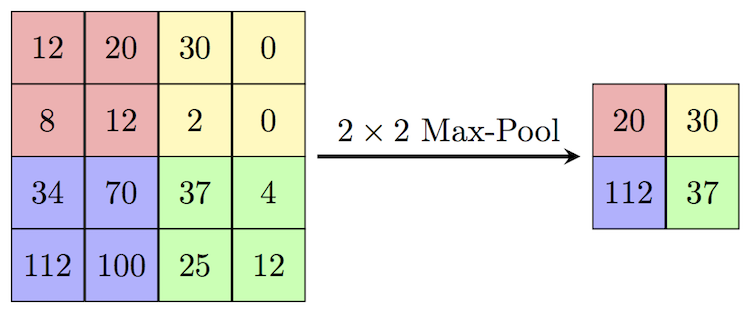
\includegraphics[width=.6\textwidth]{fig/L2/MaxpoolSample2.png}
\end{figure}
\end{frame}

\begin{frame}[fragile]{A traditionnal CNN architecture}
    \begin{figure}
\centering
    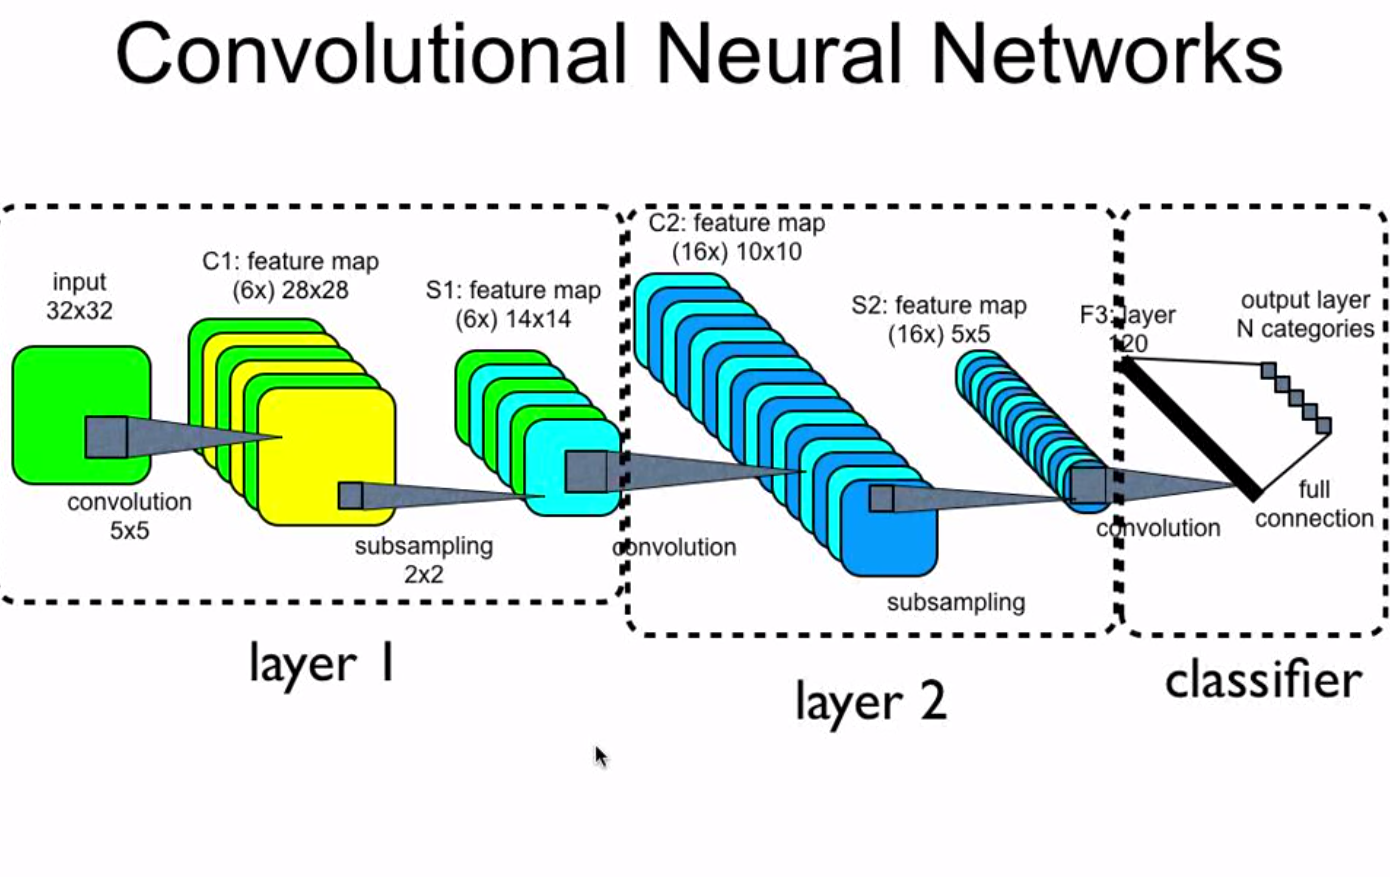
\includegraphics[width=.8\textwidth,trim={0 0cm 0cm 3cm},clip]{fig/L2/CNN.png}
\end{figure}
\end{frame}

\begin{frame}{Example of AlexNet}
    \alert{AlexNet} is the first Deep architecture used on ImageNet challenge in 2012 and achieved an \alert{error of 15.3\%} (10\% better than the previous best classifier). The paper was cited more than 34,000 times.

\begin{thebibliography}{GBC16}

\bibitem[KH12]{Krizhevsky2012ImageNetNetworks}
Alex Krizhevsky and Geoffrey~E Hinton, \emph{{ImageNet Classification with Deep
  Convolutional Neural Networks}}, Neural Information Processing Systems
  (2012), 1--9.

\end{thebibliography}
    \begin{figure}
        \centering
        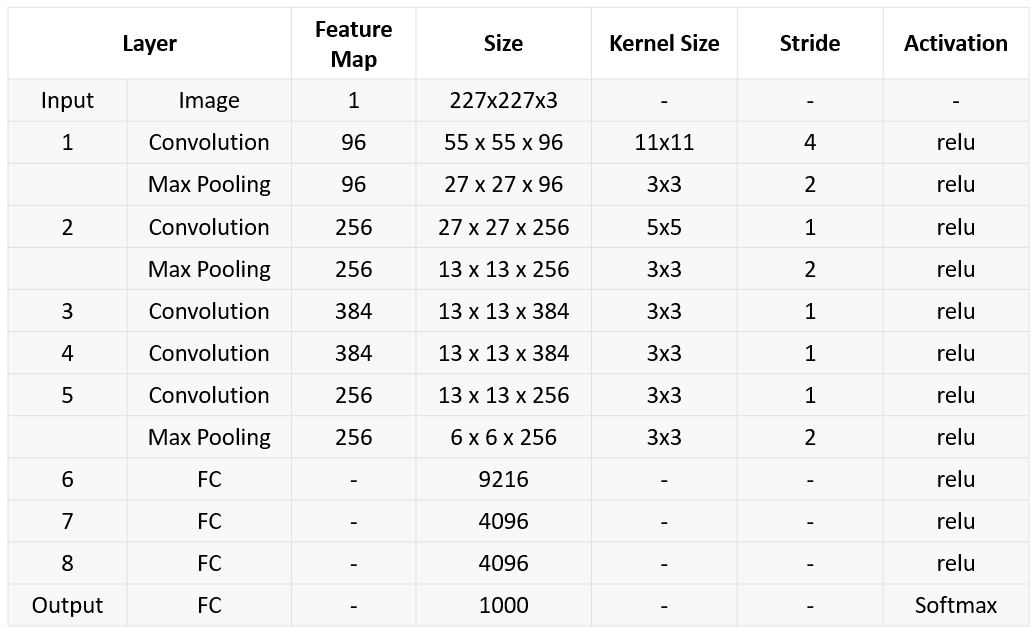
\includegraphics[width=.5\textwidth]{fig/L2/AlexNet_Summary_Table.jpg}

    \end{figure}
\end{frame}
\section{A quick typology of few neural nets}
%%%%%%%%%%%%%%%%%%%%%
\begin{frame}{Recurrent Neural Networks}
    \begin{figure}
        \centering
        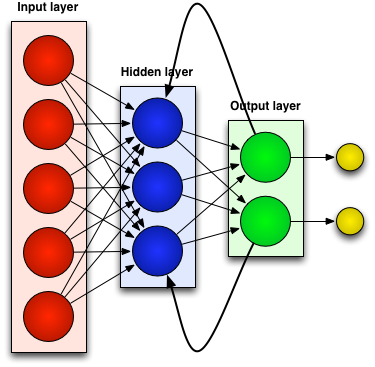
\includegraphics[width=.4\textwidth]{fig/L2/rnn.png}

    \end{figure}

Some popular types of recurrent neural networks:
\begin{itemize}
    \item Long short-term memory (LSTM)
    \item Gated Reccurent Unit (GRU)
\end{itemize}
\alert{Used in machine translation and text processing}
\end{frame}

\begin{frame}{Autoencoders}
    \begin{figure}
        \centering
        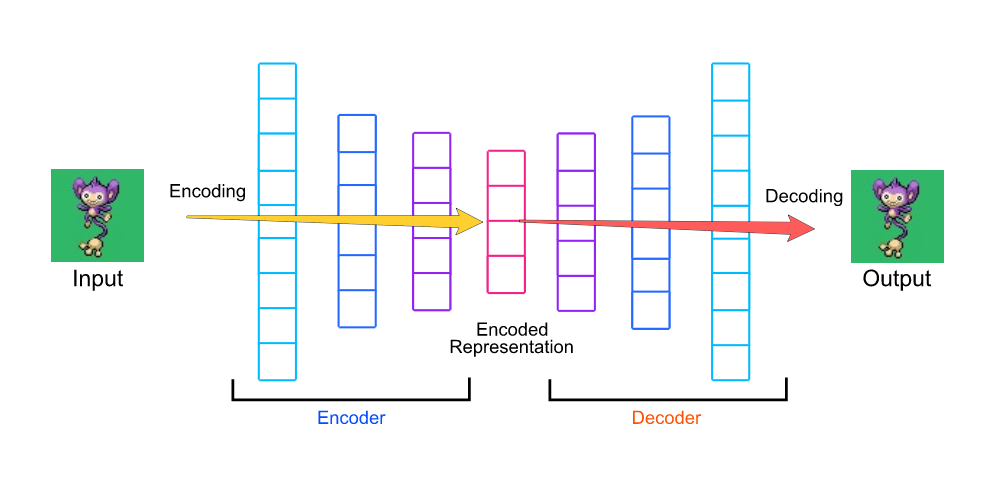
\includegraphics[width=.9\textwidth]{fig/L2/AE.png}

    \end{figure}
\alert{Used in image denoising, compressing, generation,...}
    
\end{frame}

\begin{frame}{Generative adversarial networks}
    \begin{figure}
        \centering
    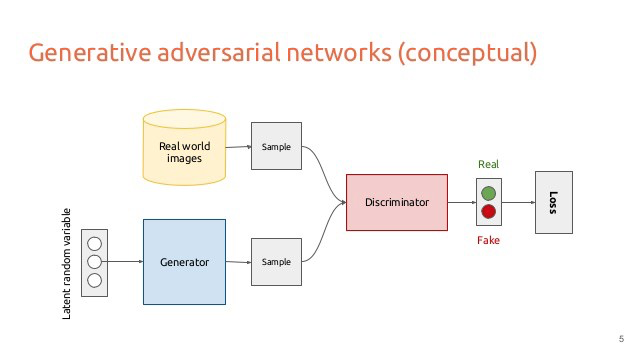
\includegraphics[width=.9\textwidth]{fig/L2/GAN.png}
  \end{figure}
    
\end{frame}

\begin{frame}{Residual Networks}
    \begin{columns}
    \column{.5\textwidth}
        \begin{figure}
        \centering
        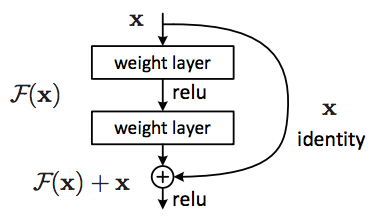
\includegraphics[width=.9\textwidth]{fig/L2/res_block.png}

    \end{figure}
    $x$~: input, $y$~: output
    $$
    y = x + \mathcal{F}(x) 
    $$
    \pause
    \column{.5\textwidth}
            \begin{figure}
        \centering
        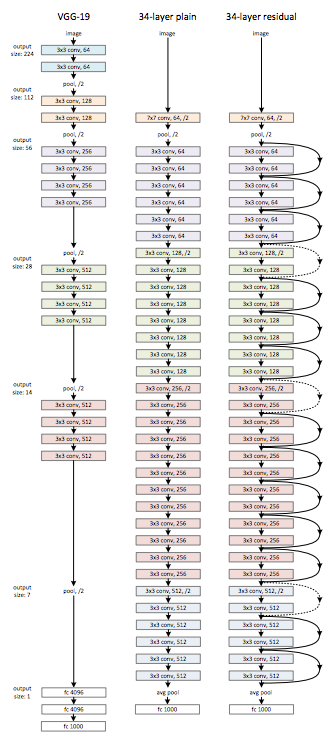
\includegraphics[height=.9\textheight,trim={4cm 0cm 0cm 0cm},clip]{fig/L2/resnet_full.png}

    \end{figure}
    \end{columns}
\end{frame}


%%%%%%%%%%%%%%%%%%
\begin{frame}[fragile]{Questions addressed in this lecture}
    \begin{itemize}
        \item What are the steps of a machine learning process? 
        \item What is the principle of the Random Forests? [Van16,5.8]
        \item How to encode qualitative features? [Van16,5.4]
        \item How to determine the hyperparamters? [Van16,5.3]
        \item What is a artificial neural network? [GBC16,6]
        \item What is a convolutive layers [GBC16,9]
            {\footnotesize
\href{https://towardsdatascience.com/intuitively-understanding-convolutions-for-deep-learning-1f6f42faee1}{https://towardsdatascience.com/intuitively-understanding-convolutions-for-deep-learning-1f6f42faee1}}
        \item What are the main types of neural networks? [GBC16,10, 14, 20]
    \end{itemize}

\begin{footnotesize}
\begin{block}{Refs}
~[Van16,$n$]: Jake VanderPlas, \textit{Python Data Science Handbook}, section $n$\\
~[GBC16,$n$]: Goodfellow etal., Deep Learning, chapter $n$
\end{block}
\end{footnotesize}
\end{frame}


\end{document}


\begin{frame}{Training a neural-net: gradient backpropagation}

\begin{columns}

\column{.5\textwidth}
\begin{figure}
    \centering
 \begin{tikzpicture}[%
    node distance = 2.5em,
    basic/.style={draw,fill=blue!20,text width=1em,text badly centered},
    input/.style={basic,circle,fill=green!20},
    output/.style={basic,circle,fill=red!20},
    weights/.style={basic,rectangle},
functions/.style={basic,circle,fill=blue!10}
]
        \node[] (center) {};
        \node[right = of center, anchor = west,output] (right) {$\hat{y}$};
        \node[above of=center,functions] (h1) {$h_1$};
        \node[below of=center,functions] (h2) {$h_2$};
        \path[draw,->] (h1) -- node[above,midway]{$w^{1}_1$}(right);
        
        \path[draw,->] (h2) --  node[below,midway]{$w^{1}_2$}(right);
        
        \node[left = of h1, input] (x1) {$x_1$};
        \node[left = of h2, input] (x2) {$x_2$};
        
        \path [draw,->] (x1) -- node[above,midway]{$w^0_{11}$} (h1);
        \path [draw,->] (x1) -- node[pos=0.25,above]{$w^0_{12}$} (h2);
        \path [draw,->] (x2) -- node[pos=0.05,above]{$w^0_{21}$} (h1);
        \path [draw,->] (x2) -- node[below,midway]{$w^0_{22}$} (h2);
\end{tikzpicture}
\end{figure}
\begin{block}{Objective}
Determination of the best set of weights $\mathbf{w}$ to minimize the Loss function $L(\mathbf{w}) = ||\hat{y}(\mathbf{w})-y||^2$.\
\alert{Calculation of $\partial L/\partial w$}
\end{block}
\column{.6\textwidth}
\begin{enumerate}[<+->]
    \item Given a couple $(x,y)$
    \item \alert{Forward computation:}\\
    $h_j  =  f_0(\sum_{i=1}^2 w^0_{ij}.x_i)$\\
$\hat{y}  =  f_1(\sum_{j=1}^2 w^1_j. h_j)$
\item \alert{Compute the gradient of the loss:~}
$\boxed{\color{red}\partial L/\partial \hat{y}}$

    \item \alert{Gradient Backpropagation:}
    \begin{itemize}
   \item Layer 1\\
   $\alert{\partial L/\partial w_j^1} = 
   \boxed{\color{red}\partial L/\partial \hat{y}}.
   \partial f_1 / \partial w^1_j$\\
   
   $ \boxed{\color{blue}\partial L/\partial h_j} = 
    \boxed{\color{red}\partial L/\partial \hat{y}}. 
   \partial f_1 / \partial h_j$
   
   \item Layer 0\\
   $\alert{\partial L/\partial w^0_{ij}}=
  \boxed{\color{blue}\partial L/\partial h_j}
   .\partial f_1 / \partial w^0_{ij}  $
    
    \end{itemize}
\end{enumerate}

\end{columns}

\end{frame}



\section{Optimizing a machine learning (gradient method)}

\begin{frame}{Optimizing the loss}
    Several loss function (depending on the problem) can be defined.
    
    For example, Mean Square Error:
    
    \begin{alertblock}{Method}
    Find a minimum of L by adjustig the parameters (weights) $\mathbf{w}$ given the gradient of the loss with respect to the weights $\nabla_\mathbf{w}L$.
    \end{alertblock}
\end{frame}

\begin{frame}{Batch gradient}
    
\end{frame}

\begin{frame}{Remarks on batch gradient}
    
\end{frame}

\begin{frame}{Scaling the data}
    
\end{frame}

\begin{frame}{Pure stochastic gradient}
    
\end{frame}

\begin{frame}{Remarks on pure stochastic gradient}
    
\end{frame}

\begin{frame}{Mini-batch gradient}
    
\end{frame}

\begin{frame}{Batch/Stochastic training}
Dataset: $(X,y)$ with N samples, $\mathbf{w}$: initial weights\\~\\
\begin{columns}[t]
\column{.5\textwidth}
\alert{Batch Training:}
\begin{itemize}
    \item For $i$ from $1$ to $N$:\\
    \begin{enumerate}
    \item    $L = L + L(f(x_i),y_i)$
     \end{enumerate}
    \item Calculate $\partial L/\partial w$
    \item update weights:$\mathbf{w}$
    
\end{itemize}
\alert{1 Update is performed after N forward passes of the neural net.}
\pause
\column{.5\textwidth}
\alert{Stochastic Training:}
\begin{itemize}
 \item For $i$ from $1$ to $N$:\\
     \begin{enumerate}

    \item Compute $L(f(x_i),y_i)$\\
    \item Calculate $\partial L/\partial w$\\
    \item update weights:$\mathbf{w}$
    \end{enumerate}
\end{itemize}

\alert{N Updates are performed after N forward passes of the neural net.}
\end{columns}
    
\end{frame}

\begin{frame}{Batch training}
Dataset: $(X,Y)$ with N samples denoted $(\mathbf{x_i},y_i)$

\begin{columns}[t]
\column{.56\textwidth}
\begin{footnotesize}
\begin{block}{Batch gradient:}\end{block}
    \begin{algorithmic}
    \Require{Learning rate(s): $\nu_k$}
    \Require{Initial weights: $\mathbf{w}$}
    \State $k \leftarrow 1$
    \While {stopping criterion not met}
   % \Require{NNNN}
    %\State Sample $m$ examples ($\mathbf{x}_i,y_i)$ from ($X,y$)
    \State Compute gradient: $\mathbf{g} \leftarrow \frac{1}{N}\sum_i^N\nabla_\mathbf{w}L(f(\mathbf{x}_i,y_i))$
    \State Update weights: $\mathbf{w} \leftarrow \mathbf{w} - \nu_k\mathbf{g}$
    \State $k \leftarrow k + 1$
    \EndWhile 
    \end{algorithmic}
    \end{footnotesize}
    \alert{1 Update / N forwards}
    \pause
    \column{.56\textwidth}
\begin{footnotesize}
\begin{block}{Stochastic gradient:}\end{block}
    \begin{algorithmic}
    \Require{Learning rate(s): $\nu_k$}
    \Require{Initial weights: $\mathbf{w}$}
    \State $k \leftarrow 1$
    \While {stopping criterion not met}
   % \Require{NNNN}
    %\State Sample $m$ examples ($\mathbf{x}_i,y_i)$ from ($X,y$)
    \State Sample an example ($\mathbf{x},y)$ from ($X,Y$)
    \State Compute gradient: $\mathbf{g} \leftarrow \nabla_\mathbf{w}L(f(\mathbf{x},y))$
    \State Update weights: $\mathbf{w} \leftarrow \mathbf{w} - \nu_k\mathbf{g}$
    \State $k \leftarrow k + 1$
    \EndWhile 
    \end{algorithmic}
    \end{footnotesize}
    \alert{1 Update / 1 forward}
    
    
    \end{columns}
\end{frame}

\begin{frame}{Mini-Bactch training}
Dataset: $(X,y)$ with N samples
\begin{footnotesize}
    \begin{algorithmic}
    \Require{Learning rate(s): $\nu_k$}
    \Require{Initial weights: $\mathbf{w}$}
    \State $k \leftarrow 1$
    \While {stopping criterion not met}
   % \Require{NNNN}
    \State Sample $m$ examples ($\mathbf{x}_i,y_i)$ from ($X,y$)
    \State Compute gradient: $\mathbf{g} \leftarrow \frac{1}{m}\sum_i^m\nabla_\mathbf{w}L(f(\mathbf{x}_i,y_i)$
    \State Update weights: $\mathbf{w} \leftarrow \mathbf{w} - \nu_k\mathbf{g}$
    \State $k \leftarrow k + 1$
    \EndWhile 
    
    \end{algorithmic}
    \end{footnotesize}
\end{frame}

\begin{frame}{Mini-Batch training}
Dataset: $(X,y)$ with N samples, $\mathbf{w}$: initial weights\\~\\
\begin{itemize}
    \item for $k$ from $1$ to  $N//B$:
\begin{itemize}
 \item for $i$ from $B(k-1)+1$ to $Bk$:\\
     \begin{enumerate}
    \item Compute $L(f(x_i),y_i)$\\
    \end{enumerate}
    \item Calculate $\partial L/\partial w$\\
    \item update weights:$\mathbf{w}$
    \end{itemize}
\end{itemize}
N//B updates are performed after N forward passes of the neural net\\
\alert{B is the batchsize}
\begin{itemize}
    \item \alert{B=1}: stochastic training
    \item \alert{B=N}: batch training
    \item Generally B<<N
\end{itemize} 

    
\end{frame}

%%%%%%%%%%%%%%%%%%%%%
%%%%%%%%%%%%%%%%%%%%%
%%%%%%%%%%%%%%%%%%%%%
%%%%%%%%%%%%%%%%%%%%%
%%%%%%%%%%%%%%%%%%%%%%%%%%%%%%%%%%%%%%%%%%
%%%%%%%%%%%%%%%%%%%%%
%%%%%%%%%%%%%%%%%%%%%%%%%%%%%%%%%%%%%%%%%%
\end{document}
%%%%%%%%%%%%%%%%%%%%%%%%%%%%%%%%%%%%%%%%%%



